%version 1.00, date 01/03/16, auteur Mathieu MEDICI, Julie PAIN

\documentclass[asi, sansVersion]{picInsa}

\usepackage{vocabulaireUnipik}

\begin{document}

\title{Description du Diagramme de classe}
\author{\Mathieu, \Julie}
\date{01/03/2016} 

\maketitle

\tableofcontents

\chapter{Diagramme de classe}

%% Inclure le  diagramme de classe
\begin{landscape}
\begin{figure}
	\centering
	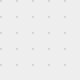
\includegraphics[scale=0.3]{images/Diagrammedeclasses}
	\caption{\label{modele}Diagramme de classe}
\end{figure}
\end{landscape}

\chapter{Description du Diagramme de classe}

Le diagramme de classe réalisé est composé de plusieurs types, de plusieurs classes et de plusieurs associations. Nous allons les décrire dans cette partie. \\ 

\section{Les types}

\subsection*{LocalisationWGS84}

Le type LOCALISATIONWGS84 est un data type qui définit la localisation en respectant la norme WGS84.

\subsection*{Theme}

Le type THEME est une énumération qui définit les différents thèmes possibles pour les plaidoyers.

\subsection*{NiveauScolaireComplet}

Le type NIVEAUSCOLAIRECOMPLET est une énumération qui définit tous les niveaux possibles pour les interventions plaidoyer. Ce type comporte aussi des combinaisons des niveaux comme par exemple "CPCE1" ou "CM1CM2". La valeur "autre" est utilisée pour des cas particuliers (niveau CLIS, CM26eme).

\subsection*{NiveauScolaireLimite}

Le type NIVEAUSCOLAIRECOMPLET est une énumération qui définit tous les niveaux possibles pour les interventions frimousse en se limitant à l'école primaire. Ce type comporte aussi des combinaisons des niveaux comme par exemple "CPCE1" ou "CM1CM2". La valeur "autre" est utilisée pour des cas particuliers (niveau CLIS, CM26eme).

\subsection*{TypeCentre}

Le type TYPECENTRE est une énumération qui définit les différents niveaux pour les centres de loisirs.

\subsection*{TypeEnseignement}

Le type TYPEENSEIGNEMENT est une énumération qui définit les différents niveaux pour les enseignements.

\subsection*{TypeProjet}

Le type TYPEPROJET est une énumération qui définit les différents niveaux pour les projets.

\subsection*{TypeContact}

Le type TYPECONTACT est une énumération qui définit les différents contacts possibles.

\subsection*{Materiel}

Le type MATERIEL est une énumération qui définit les différents types de matériel possibles pour une intervention.

\subsection*{MaterielFrimousse}

Le type MATERIELFRIMOUSSE est une énumération qui définit les différents matériaux possibles pour les interventions frimousses.

\subsection*{Activite}

Le type ACTIVITE est une énumération qui définit les différentes activités que peuvent réaliser les bénévoles.

\subsection*{MomentHebdomadaire}

Le type MOMENTHEBDOMADAIRE est une énumération qui définit les différents moments possibles dans une semaine, un moment étant soit le matin soit l'après-midi.

\subsection*{MomentQuotidien}

Le type MOMENTQUOTIDIEN est une énumération qui définit les différents moments possibles dans une journée, donc matin ou après-midi.

\subsection*{NiveauTheme}

La classe NIVEAUTHEME définit un type qui est la combinaison d'un thème et d'un niveau.\\
Cette classe a plusieurs attributs : 
\begin{itemize}
\item un niveau qui appartient à l'énumération NIVEAUSCOLAIRECOMPLET;
\item un thème qui appartient à l'énumération THEME.
\end{itemize}

\subsection*{Semaine}

La classe SEMAINE définit un type qui est une semaine du calendrier.\\
Cette classe a un attribut : 
\begin{itemize}
\item un identifiant unique.
\end{itemize}

\subsection*{Adresse}

La classe ADRESSE définit un type qui est l'adresse d'une personne ou d'un établissement.\\
Cette classe a plusieurs attributs : 
\begin{itemize}
\item une rue;
\item un numéro de rue avec si besoin le supplément "bis", "ter" ou "quater";
\item un code postal;
\item une ville;
\item un complément si besoin.
\end{itemize}

\section{Les classes}

\subsection*{Personne}

La classe PERSONNE est la classe mère des classes BENEVOLE et CONTACT. C'est une généralisation, c'est à dire que la classe PERSONNE est une classe abstraite et donc une PERSONNE est soit un contact, soit un bénévole. \\
Cette classe a plusieurs attributs : 
\begin{itemize}
\item un nom; %Cdc - Non NULL
\item un prénom; %Cdc - Non NULL
\item un numéro de téléphone fixe; %Cdc - Peut être NULL
\item un numéro de téléphone portable; %Cdc - Peut être NULL
\item un email. %Ne peut pas être NULL (Clé)
\end{itemize}

\subsection*{Benevole}

La classe BENEVOLE est une classe fille de la classe PERSONNE et la classe mère des classes ADMINLOCAL et ADMINGLOBAL. Cette classe décrit les bénévoles de l'UNICEF qui réaliseront des interventions mais aussi ceux qui géreront des activités (ADMINLOCAL) ou des départements (ADMINGLOBAL). L'héritage est ici une spécialisation, c'est à dire qu'une personne peut être simplement bénévole sans être ni administrateur global, ni administrateur local. \\
Cette classe a plusieurs attributs : 
\begin{itemize}
\item une adresse correspondant à la rue, au numéro de rue, au code postal, à la ville et au complément si besoin; %Adresse est une classe
\item aucune, une ou plusieurs activités potentielles (action ponctuelle, frimousse, plaidoyer); % attribut multivalué
\item un mot de passe. 
\end{itemize}

\subsection*{AdminLocal}

La classe ADMINLOCAL permet de représenter un administrateur local. Cette classe est une classe fille de la classe BENEVOLE.\\
Cette classe a un attribut :
\begin{itemize}
\item aucune, une ou plusieurs responsabilités d'activité (action ponctuelle, frimousse, plaidoyer). 
\end{itemize}

\subsection*{AdminGlobal}

La classe ADMINGLOBAL permet de représenter un administrateur global. Cette classe est une classe fille de la classe BENEVOLE. 

\subsection*{Contact}

La classe CONTACT est une classe fille de la classe PERSONNE. Cette classe décrit les personnes étant reliées à un établissement comme le personnel y travaillant ou encore les élèves. \\
Cette classe a un attribut : 
\begin{itemize}
\item un type de contact qui permet de déterminer si un contact est un enseignant, un animateur, un contact frimousse, un contact plaidoyer, un contact activité ponctuelle ou un responsable d'établissement.
\end{itemize} 


\subsection*{Etablissement}

La classe ETABLISSEMENT est la classe mère des classes ENSEIGNEMENT et CENTRELOISIRS. C'est une généralisation, c'est à dire que la classe ETABLISSEMENT est une classe abstraite et donc un établissement est soit un enseignement, soit un centre de loisirs. \\
Cette classe a plusieurs attributs : 
\begin{itemize}
\item un identifiant unique;
\item un nom;
\item une adresse correspondant à la rue, au numéro de rue, au code postal, à la ville et au complément si besoin; %Adresse est une classe
\item un numéro de téléphone fixe;
\item une ou plusieurs adresses e-mail; % attribut multivalué
\item une géolocalisation WGS84. % Peut être NULL
\end{itemize}

\subsection*{Enseignement}
La classe ENSEIGNEMENT est une classe fille de la classe ETABLISSEMENT. Cette classe décrit les établissements qui relèvent de l'éducation nationale. \\
Cette classe a plusieurs attributs : 
\begin{itemize}
\item un UAI (Unité Administrative Immatriculée) qui est une combinaison de chiffres et de lettres unique pour chaque enseignement;
\item un type d'enseignement qui permet de déterminer si l'enseignement est une école maternelle, une école élémentaire, un collège, un lycée ou un établissement supérieur. 
\end{itemize} 


\subsection*{Centre de loisirs}
La classe CENTRELOISIRS est une classe fille de la classe ETABLISSEMENT. Cette classe décrit les établissements ayant un rapport avec les loisirs. \\
Cette classe a un attribut : 
\begin{itemize}
\item un type de centre de loisirs qui permet de déterminer si un centre de loisirs prend en charge des enfants d'école maternelle, d'école élémentaire ou des adolescents.
\end{itemize}  

\subsection*{Intervention}
La classe INTERVENTION est la classe mère des classes PLAIDOYER et FRIMOUSSE. Cette classe décrit une intervention que peut demander un établissement ou un contact. \\
Cette classe a plusieurs attributs :
\begin{itemize}
\item un identifiant unique;
\item une date précise déterminée par les bénévoles lors de l'attribution des bénévoles aux interventions;
\item un moment indiquant si l'intervention a lieu le matin ou l'après-midi;
\item le nombre de personnes concernées par cette intervention (exemple : le nombre d'élève d'une classe);
\item le matériel disponible pour l'intervention (présence ou non d'un rétroprojecteur, d'un tableau intéractif ou d'enceintes);
\item un lieu dans l'établissement, c'est à dire la salle où aura lieu l'intervention;
\item un champ remarque permettant à l'utilisateur de saisir des remarques spécifiques à cette intervention. 
\end{itemize}

\subsection*{Plaidoyer}
La classe PLAIDOYER est une classe fille de la classe INTERVENTION. \\
Cette classe a un attribut : 
\begin{itemize}
\item un niveau-thème qui indique à la fois le thème de l'intervention et le niveau de la classe dans laquelle va se dérouler l'intervention, par exemple, pour une école primaire, la classe peut être CE1 mais aussi CE1-CE2.
\end{itemize}

\subsection*{Frimousse}
La classe FRIMOUSSE est une classe fille de la classe INTERVENTION. Une activité frimousse est réalisée avec des enfants d'école élémentaire. \\
Cette classe a plusieurs attributs :
\begin{itemize}
\item les matériaux nécessaires à la réalisation de l'activité (patron, bourre, décoration); % Attribut multivalué
\item un niveau qui correspond à la classe dans laquelle va se dérouler l'intervention (CP, CE1, etc).
\end{itemize}

\subsection*{Projet}
La classe PROJET représente les projets réalisées par des étudiants ou des lycéens.\\
Cette classe a plusieurs attributs : 
\begin{itemize}
\item un identifiant unique;
\item le type de projet permet de savoir si le projet est réalisé par des étudiants, des lycéens, des élèves d'école primaire ou de collège; 
\item la description du projet est un champ permettant à l'utilisateur de saisir toutes les informations importantes sur le projet (le nom du projet, s'il y a un tuteur);
\item le chiffre d'affaire réalisés par ce projet.
\end{itemize}

\subsection*{Vente}
La classe VENTE représente les actions ponctuelles réalisées par les établissements.\\ 
Cette classe a plusieurs attributs : 
\begin{itemize}
\item un identifiant unique; 
\item le chiffre d'affaire réalisés par cette vente;
\item la date de la vente;
\item un champ remarques permettant à l'utilisateur d'ajouter des informations importantes. 
\end{itemize}

\subsection*{Demande}

La classe DEMANDE représente les demandes d'intervention effectuées par les contacts.\\
Cette classe a plusieurs attributs :
\begin{itemize}
\item un identifiant unique; 
\item une liste des semaines correspondant aux semaines où le contact est disponible; 
\item les moments voulus pour une semaine type (sera donc valable pour toutes les semaines où le contact est disponible);
\item les moments à éviter pour une semaine type. 
\end{itemize}

\subsection*{Departement}

La classe DEPARTEMENT représente les départements français.\\
Cette classe a plusieurs attributs :
\begin{itemize}
\item un identifiant unique (le numéro du département). 
\end{itemize}


\section{Les associations}

\subsection*{estResponsable}
L'association ESTRESPONSABLE relie un BENEVOLE et un PROJET. Un benévole est responsable d'aucun, un ou plusieurs projets et un projet est sous la responsabilité d'aucun (si le projet est en attente), un ou plusieurs bénévoles.

\subsection*{participe}
L'association PARTICIPE relie un CONTACT et un PROJET. Un contact participe à aucun, un ou plusieurs projets et un projet a pour participant aucun (si le projet est en attente), un ou plusieurs contacts.\\
Cette association a un attribut :
\begin{itemize}
\item un booléen qui indique si le contact est ou non un tuteur du projet (un professeur tuteur des élèves réalisant le projet par exemple). 
\end{itemize}

\subsection*{realise}

L'association REALISE est une association ternaire qui relie une VENTE, un ETABLISSEMENT et une INTERVENTION. Un établissement réalise aucune, une ou plusieurs ventes. Une vente est réalisée par un et un seul établissement. La vente est à l'origine d'aucune ou une intervention.

\subsection*{fait}

L'association FAIT relie un CONTACT et une DEMANDE. Un contact fait aucune, une ou plusieurs demandes, une demande est faite par un et un seul contact.

\subsection*{cree}

L'association CREE relie une DEMANDE et une INTERVENTION. Une demande crée une ou plusieurs interventions, une intervention est créée par une et une seule demande.

\subsection*{effectue} 

L'association EFFECTUE relie un BENEVOLE et une INTERVENTION. Un bénévole effectue aucune, une ou plusieurs interventions. Une intervention est effectuée par un et un seul utilisateur. 

\subsection*{Appartient}

L'association APPARTIENT relie un CONTACT et un ETABLISSEMENT. Un contact appartient à aucun, un ou plusieurs établissements. Un établissement a un ou plusieurs contacts.\\
Cette association a plusieurs attributs :
\begin{itemize}
\item un booléen qui indique si le contact est ou non le responsable de l'établissement; 
\item un type qui indique si le contact est responsable d'aucune, une ou plusieurs activités.
\end{itemize}

\subsection*{effectuerDans}

L'association ESTEFFECTUEDANS relie une INTERVENTION et un ETABLISSEMENT. Une intervention est effectuée dans un et un seul établissement, un établissement peut être le lieu d'aucune, une ou plusieurs interventions.

\subsection*{benevoleSeSitue}

L'association BENEVOLESESITUE relie un BENEVOLE et un DEPARTEMENT. Un bénévole se situe dans un et un seul département, un département a aucun, un ou plusieurs bénévoles.

\subsection*{interventionSeSitue}

L'association INTERVENTIONSESITUE relie une INTERVENTION et un DEPARTEMENT. Une intervention se situe dans un et un seul département, un département a aucune, une ou plusieurs interventions.

\subsection*{estAssocie}

L'association ESTASSOCIE relie un DEPARTEMENT à lui-même. Un département est associé à aucun, un ou plusieurs départements.

\chapter{Contraites d'intégrité}

\section{Les contraintes d'intégrité intra-classe}
Dans cette partie, nous allons décrire les différentes contraintes d'intégrité de chaque classe et classe-association.
 
\subsection*{Personne}
Contraintes de domaine et de nullité des attributs :
\begin{itemize}
 	\item \textbf{nom :} chaine de caractère de longueur de 100 caractères au maximum, attribut non nul;
	\item \textbf{prénom :} chaine de caractère de longueur de 100 caractères au maximum, attribut non nul;
	\item \textbf{email :} chaine de caractère de longueur de 100 caractères au maximum, la syntaxe de l'e-mail doit être la suivante : user@host.domain\\
	user : contient des chiffres/lettres ainsi que les symboles "\_", "-", "." \\
	host : contient des chiffres/lettres \\
	domain : chaine de caractère composée de 2 ou 3 lettres. \\
	attribut non nul;  
	\item \textbf{telFixe :} chaine de caractère composée de 10 chiffres commençant par "0", attribut peut être nul;
	\item \textbf{telPortable :} chaine de caractère composée de 10 chiffres commençant par "0", attribut peut être nul.\\
\end{itemize}  

\subsection*{Benevole}
Contraintes de domaine et de nullité des attributs :
\begin{itemize}
 	\item \textbf{adresse :} constante de type \textbf{Adresse}, attribut non nul;
	\item \textbf{mdp :} chaine de caractère de longueur de 50 caractères au maximum, de 8 caractères au minimum, attribut non nul;  
	\item \textbf{activitesPotentielles :} constante de type \textbf{Activite}, atrribut multivalué, peut être nul.\\
\end{itemize}  

\subsection*{AdminLocal}
Contraintes de domaine et de nullité des attributs :\\
 \indent \indent \textbf{responsabiliteActivite :} constante de type \textbf{Activite}, attribut multivalué, peut être nul.\\

 
\subsection*{Contact}
Contraintes de domaine et de nullité des attributs :\\
\indent \indent \textbf{type :} constante de type \textbf{TypeContact},attribut non nul.\\

\subsection*{Etablissement}
Contraintes de domaine et de nullité des attributs :
\begin{itemize}
 	\item \textbf{idEtablissement :} chaine de caractère de longueur de 100 caractères au maximum, attribut non nul;
	\item \textbf{nom :} chaine de caractère de longueur de 100 caractères au maximum, attribut non nul;
	\item \textbf{telFixe :} chaine de caractère composée de 10 chiffres commençant par "0", attribut peut être nul;
	\item \textbf{email :} chaine de caractère de longueur de 100 caractères au maximum, la syntaxe de l'e-mail doit être la suivante : user@host.domain\\
	user : contient des chiffres/lettres ainsi que les symboles "\_", "-", "." \\
	host : contient des chiffres/lettres \\
	domain : chaine de caractère composée de 2 ou 3 lettres. \\
	attribut multivalué, non nul; 
	\item \textbf{adresse :} constante de type \textbf{Adresse}, attribut non nul; 
	\item \textbf{geolocalisation :} constante de type \textbf{LocalistaionWGS84}, attribut non nul.\\
\end{itemize}  

\subsection*{Enseignement}
Contraintes de domaine et de nullité des attributs :
\begin{itemize}
	\item \textbf{UAI :} chaine de caractères composée de lettre et de chiffres, attribut non nul;
	\item \textbf{type :} constante de type \textbf{TypeEnseignement}, attribut non nul.\\
\end{itemize}

\subsection*{Centre de Loisirs}
Contraintes de domaine et de nullité des attributs :\\
\indent \indent \textbf{type :} constante de type \textbf{TypeCentre}, peut être nul.\\

\subsection*{Intervention} 
Contraintes de domaine et de nullité des attributs :
\begin{itemize}
 	\item \textbf{idIntervention :} entier, attribut non nul;
	\item \textbf{date :} chaine de caractère de longueur de 10 caractères ayant la syntaxe suivante "JJ/MM/AAAA", attribut non nul;
	\item \textbf{lieu :} chaine de caractère composée de chiffres et de lettres, attribut peut être nul;
	\item \textbf{nbPersonnes :} entier, attribut non nul;  
	\item \textbf{materielDispo :} constante de type \textbf{Matériel}, attribut multivalué non nul; 
	\item \textbf{remarques :} chaine de caractères de longueur de 1000 caractères au maximum;
	\item \textbf{moment :} constante de type \textbf{MomentJournalier}, attribut peut être nul;\\
\end{itemize}  

\subsection*{Plaidoyer}
Contraintes de domaine et de nullité des attributs :\\
\indent \indent \textbf{niveauThème :} constante de type \textbf{niveauThème}, attribut non nul.\\

\subsection*{Frimousse}
Contraintes de domaine et de nullité des attributs :
\begin{itemize}
	\item \textbf{materiaux :} constante de type \textbf{MaterielFrimousse}, attribut multivalué non nul;
	\item \textbf{niveaux :} constante de type \textbf{NiveauScolaireLimite}, attribut non nul.\\
\end{itemize}

\subsection*{Projet}
Contraintes de domaine et de nullité des attributs :
\begin{itemize}
 	\item \textbf{idProjet :} entier, attribut non nul;
	\item \textbf{chiffreDAffaire :} Entier, attribut non nul;
	\item \textbf{description :} chaine de caractère composée de longueur de 1000 caractères au maximum, attribut ne peut être nul;
	\item \textbf{type :} constante de type \textbf{TypeProjet}, attribut non nul. \\  
\end{itemize} 

\subsection*{Vente}
Contraintes de domaine et de nullité des attributs :
\begin{itemize}
 	\item \textbf{idVente :} entier, attribut non nul;
	\item \textbf{chiffreDAffaire :} Entier, attribut non nul;
	\item \textbf{date :} chaine de caractère de longueur de 10 caractères ayant la syntaxe suivante "JJ/MM/AAAA", attribut non nul;
	\item \textbf{remarques :} chaine de caractères de longueur de 1000 caractères au maximum. \\  
\end{itemize} 

\subsection*{Demande}
Contraintes de domaine et de nullité des attributs :
\begin{itemize}
 	\item \textbf{idDemande :} entier, attribut non nul;
	\item \textbf{momentsVoulus :} constante de type \textbf{MomentHebdomadaire}, attribut multivalué non nul;
	\item \textbf{momentsVoulus :} constante de type \textbf{MomentHebdomadaire}, attribut multivalué non nul;
	\item \textbf{date :} chaine de caractère de longueur de 10 caractères ayant la syntaxe suivante "JJ/MM/AAAA", attribut non nul. \\
\end{itemize} 

\subsection*{Departement}
Contraintes de domaine et de nullité des attributs :
\begin{itemize}
	\item \textbf{idDepartement :} Entier, attribut non nul;
	\item \textbf{nom :} chaine de caractère de longueur de 100 caractères au maximum, attribut non nul.\\
\end{itemize}

\subsection*{Adresse}
Contraintes de domaine et de nullité des attributs :
\begin{itemize}
 	\item \textbf{ville :} chaine de caractère de longueur de 100 caractères au maximum, attribut non nul;
	\item \textbf{rue :} chaine de caractère de longueur de 500 caractères au maximum, attribut non nul;
	\item \textbf{numeroDeRue :} chaine de caractère composée d'un numéro et, si besoin, de "bis", "ter", "quater", attribut non nul; 
	\item \textbf{complement : } chaine de caractère de longueur de 100 caractères au maximum;
	\item \textbf{codePostale :} chaine de caractère composée de 5 chiffres, attribut non nul.\\
\end{itemize}

\subsection*{NiveauTheme}
Contraintes de domaine et de nullité des attributs :
\begin{itemize}
	\item \textbf{niveau :} constante de type \textbf{NiveauScolaireComplet}, attribut non nul;
	\item \textbf{theme :} constante de type \textbf{Theme}, attribut non nul.\\
\end{itemize}

Autres contraintes :

Si le niveau est "petiteSection", "petiteMoyenneSection", "moyenneSection", "moyenneGrandeSection", "grandeSection", ou "petiteMoyenneGrandeSection", le thème associé doit être un des thèmes suivants : "conventionInternationaleDesDroitsDeLEnfant", "education", "laSanteAlimentation", "eau" et "harcelement". 

Si le niveau est "CP", "CPCE1", "CE1", "CE1CE2", "CE2", "CE2CM1", "CM1", "CM1CM2" ou "CM2", le thème associé doit être un des thèmes suivants : "conventionInternationaleDesDroitsDeLEnfant", "education", "laSanteEnGeneral", "santeAlimentation", "eau", "travailDesEnfants" et "harcelement".

Si le niveau est "6eme", "5eme", "4eme" ou "3eme", le thème associé doit être un des thèmes suivants : "conventionInternationaleDesDroitsDeLEnfant", "education", "laSanteEnGeneral", "santeAlimentation", "eau", "urgencesMondiales", "travailDesEnfants", "enfantsSoldats" et "harcelement".

Si le niveau est "2nde", "1ere", "terminale", "L1", "L2", "L3", "M1", "M2" ou "autre" le thème associé doit être un des thèmes suivants : "conventionInternationaleDesDroitsDeLEnfant", "education", "laSanteEnGeneral", "santeAlimentation", "vihSida", "eau", "urgencesMondiales", "travailDesEnfants", "enfantsSoldats", "harcelement", "roleDeLUnicef" et "millenairePourLeDeveloppement".\\

\subsection*{Participe}
Contraintes de domaine et de nullité des attributs :\\
\indent \indent \textbf{estTuteur :} Booléen, attribut non nul.\\


\subsection*{Appartient}
Contraintes de domaine et de nullité des attributs :
\begin{itemize}
	\item \textbf{respoEtablissement :} , attribut non nul;
	\item \textbf{type :} constante de type \textbf{Activite}, attribut multivalué peut être nul.
\end{itemize}

\section{Les contraintes d'intégrités inter-classe}

\subsection*{Etablissement - Enseignement}
L'\textbf{idEtablissement} d'un établissement doit correspondre à l'\textbf{UAI} si cette établissement est une instance d'enseignement.\\

\subsection*{Intervention - Plaidoyer}
Le \textbf{niveau} d'une intervention frimousse ainsi que le \textbf{niveau} (de NiveauTheme) d'une intervention plaidoyer doit être en correspondance avec le \textbf{type} de l'établissement.  

Si l'établissement est un enseignement, le \textbf{niveau} peut prendre différentes valeurs selon le \textbf{type}:
\begin{itemize}
\item Si le \textbf{type} est "maternelle", le \textbf{niveau} peut être : "petiteSection", "petiteMoyenneSection", "moyenneSection", "moyenneGrandeSection", "grandeSection", "petiteMoyenneGrandeSection" ou "autre";
\item Si le \textbf{type} est "elementaire", le \textbf{niveau} peut être : "CP", "CPCE1", "CE1", "CE1CE2", "CE2", "CE2CM1", "CM1", "CM1CM2", "CM2" ou "autre";
\item Si le \textbf{type} est "college", le \textbf{niveau} peut être : "6eme", "5eme", "4eme", "3eme" ou "autre";
\item Si le \textbf{type} est "lycee", le \textbf{niveau} peut être : "2nde", "1ere", "terminale" ou "autre";
\item Si le \textbf{type} est "superieur", le \textbf{niveau} peut être : "L1", "L2", "L3", "M1", "M2" ou "autre".
\end{itemize}

Si l'établissement est un centre de loisirs, le \textbf{niveau} peut prendre différentes valeurs selon le \textbf{type}:
\begin{itemize}
\item Si le \textbf{type} est "maternelle", le \textbf{niveau} peut être : "petiteSection", "petiteMoyenneSection", "moyenneSection", "moyenneGrandeSection", "grandeSection", "petiteMoyenneGrandeSection" ou "autre";
\item Si le \textbf{type} est "elementaire", le \textbf{niveau} peut être : "CP", "CPCE1", "CE1", "CE1CE2", "CE2", "CE2CM1", "CM1", "CM1CM2", "CM2" ou "autre";
\item Si le \textbf{type} est "adolescent", le \textbf{niveau} peut être : "6eme", "5eme", "4eme", "3eme", "2nde", "1ere", "terminale" ou "autre".
\end{itemize}


\end{document}